\graphicspath{{04_interpretation/figures/}} % Location of the graphics files

\chapter{Interpretation Based on Reference Resolution}
\label{04_chp:interpretation}

Interpreting the process of common grounding is a challenging task, especially under continuous and partially-observable context where complex ambiguity, uncertainty, partial understandings and misunderstandings are introduced. Interpretation becomes even more challenging when we deal with existing dialogue systems which still have limited capability of natural language understanding and generation. To address this problem, we consider reference resolution as the central subtask of common grounding and propose a new resource to study its intermediate process. Based on a simple and general annotation schema, we collected a total of 40,172 referring expressions in 5,191 dialogues curated from OneCommon Corpus, along with multiple judgements of referent interpretations. We show that our annotation is highly reliable, captures the complexity of common grounding through a natural degree of reasonable disagreements, and allows for more detailed and quantitative analyses of common grounding strategies. Finally, we demonstrate the advantages of our annotation for interpreting, analyzing and improving common grounding in baseline end-to-end dialogue systems.

\section{Introduction}
\label{04_sec:introduction}

Common grounding is the process of creating, repairing and updating mutual understandings, which is a critical aspect of sophisticated human communication \citep{clark1996using} as well as a longstanding goal in dialogue modeling \citep{traum1994computational}. Recently, there have been new proposals of dialogue tasks which require advanced skills of common grounding under \textit{continuous} and \textit{partially-observable} context \citep{udagawa2019natural,haber-etal-2019-photobook}. Their main contributions include the establishment of clear evaluation metrics (based on task success rates), collection of large-scale datasets and introduction of complex ambiguity, uncertainty, partial understandings and misunderstandings which are minimally observed under traditional (either categorical or fully-observable) context.

However, interpretation of the process of common grounding remains an open problem. Although formal approaches such as \citet{lascarides2009agreement} and \citet{poesio2010completions} account for some of the important details in common grounding, constructing such precise semantic representations is a difficult and costly process, especially under continuous and partially-observable context with high ambiguity and uncertainty. Interpretation becomes even more challenging when we deal with existing dialogue systems represented by the end-to-end dialogue systems \citep{vinyals2015neural,bordes2017learning}, which can converse fluently but still lack the true competence of natural language understanding and generation.

In this study, we approach this problem by \textit{decomposing} the common grounding task based on its intermediate subtasks. Specifically, we consider \textit{reference resolution} as the central subtask of common grounding (in the sense that mutual understanding can only be created through successful references), define this subtask formally based on a simple and general annotation schema, and create a large-scale resource to study this subtask along with the original task of common grounding.

Our annotated corpus consists of a total of 40,172 referring expressions in 5,191 dialogues curated from OneCommon Corpus \citep{udagawa2019natural}, along with multiple (a minimum of 3) judgements for referent interpretations. A visualization of our annotation is shown in Figure \ref{04_fig:first_example}.

\begin{figure*}[th!]
\centering
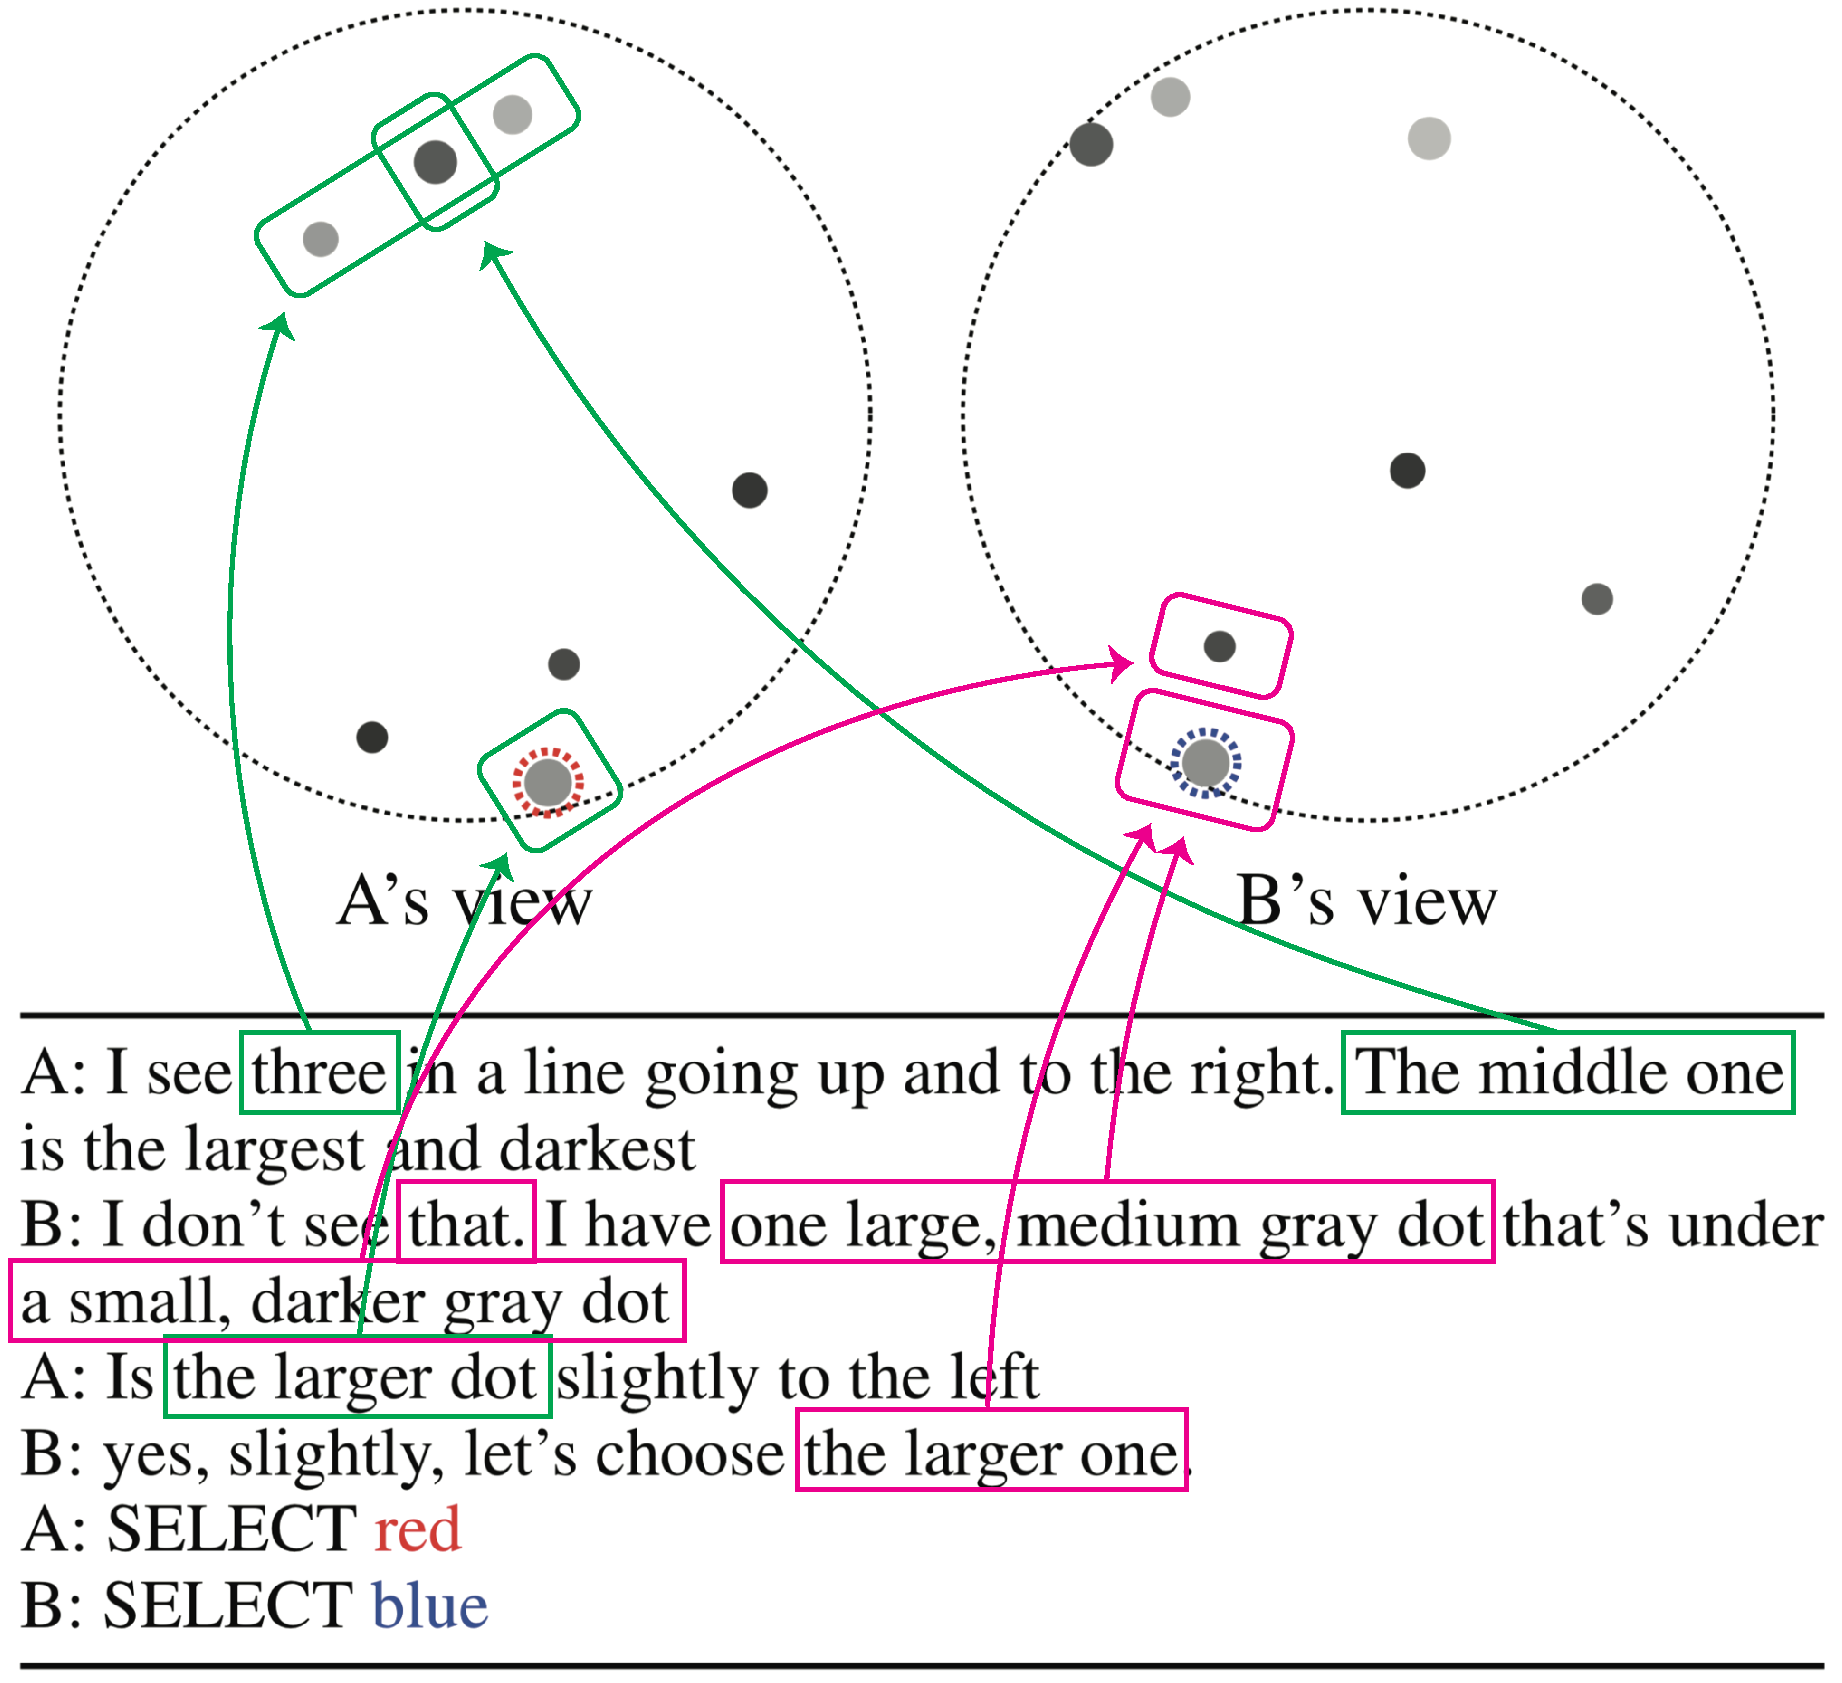
\includegraphics[width=0.7\textwidth]{annotated_dialogue.pdf}
\caption{A visualized example of our annotation. We identify all referring expressions in the dialogue and their intended referents based on the speaker's perspective (only one judgement shown in this example).
}
\label{04_fig:first_example}
\end{figure*}

Through our corpus analyses, we show that our annotation has high agreement in general but also includes a natural degree of reasonable disagreements, which verified that our annotation can be conducted reliably while capturing the ambiguity and uncertainty under continuous and partially-observable context. In addition, we give a more quantitative analysis of \textit{pragmatic expressions} as an illustrative example of analyses that can be conducted based on our annotation.

Finally, in our experiments, we show that our annotation is critical for interpreting and analyzing common grounding in baseline end-to-end dialogue systems, as well as improving their performance on difficult end tasks.

Overall, the contributions of this chapter are as follows:

\begin{itemize}
  \item We proposed a novel method of decomposing common grounding based on the central subtask of \textit{reference resolution} to study the intermediate process of common grounding.
  \item We conducted a large-scale annotation of 5,191 dialogues from OneCommon Corpus, including 40,172 referring expressions with multiple judgements for referent identification.
  \item We verified the \textit{reliability} of our annotation (while capturing genuine ambiguity based on reasonable disagreements) as well as the \textit{usefulness} for analyzing human common grounding strategies.
  \item Our experiments demonstrate that our annotation can be utilized for both interpreting and improving common grounding in end-to-end dialogue systems.
\end{itemize}

\section{Annotation Procedure}
\label{04_sec:annotation_procedure}

The goal of our annotation is to provide a \textit{general}, \textit{reliable} and \textit{useful} annotation of reference resolution to study the intermediate process of common grounding. In this work, we use the 5,191 dialogues in OneCommon Corpus which succeeded on the collaborative reference task, since they are expected to be of higher quality (c.f. Section \ref{03_subsec:results}). Our annotation procedure consists of two main steps: \textit{markable detection} to semi-automatically detect the referring expressions under consideration, followed by \textit{referent identification} to identify their referents.

As an optional step, we also conducted \textit{preprocessing} of the dialogues to correct obvious misspellings and grammatical errors. Due to the limited size of the vocabulary, we manually looked for rare unigrams and bigrams in the dialogue and carefully designed rules to correct them. Our preprocessing step is reversible, so the collected annotation can also be applied to the original dialogues without preprocessing.

\subsection{Step 1: Markable Detection}
\label{04_subsec:markable_detection}

In this study, we define a \textit{markable} to be an independent referring expression of the entities under consideration: in our case, the synthetic entities on the 2-D plane. Basically, we annotate a markable as a minimal noun phrase including all prenominal modifiers (such as determiners, quantifiers, and adjectives) but excluding all postnominal modifiers (such as prepositional phrases and relational clauses). This eliminates the complexity of the annotation because markables will not overlap or nest with each other.
%See the figures for many examples of the detected markables.

To reduce the annotation effort in the later process, we optionally annotate three attributes for each markable if they are obvious from the context: a \textit{generic} attribute when the markable is not specific enough to identify the referents, \textit{all-referents} when the markable is referring to all of the entities in the speaker's view, and \textit{no-referent} when the referents are empty. \textit{Generic} markables are ignored in our annotation, and the referents of \textit{all-referents} or \textit{no-referent} are annotated automatically in the later process. To reduce the redundancy of annotation, we consider a predicative noun phrase as a markable only if there is no previous markable in the same utterance that refers to the same entities: for example, ``\textit{a triangle}'' in ``\underline{three dots} are forming \textit{a triangle}'' is not considered as a markable since ``three dots'' is already annotated, but it is considered a markable in ``\underline{one light dot} and \underline{two dark dots} are forming \underline{\textit{a triangle}}'' (underlines indicate markables). We also annotate obvious \textit{anaphoric} and \textit{cataphoric} relations in the same utterance if they have identical referents: this way, the referents of anaphoric/cataphoric markables can be annotated automatically based on their antecedents/postcedents. However, we do not annotate such relations \textit{across utterances} as they can potentially refer to different entities, e.g. in the case of misunderstandings (as shown in Figure \ref{04_fig:misunderstanding_partial_understanding}).

The annotators were graduate students with sufficient experience and training, and we used the brat annotation tool \citep{stenetorp2012brat} to detect the markables, their attributes and relations. All available information were accessible during the annotation, including the original dialogues, players' observations and final selections.

\subsection{Step 2: Referent Identification}
\label{04_subsec:referent_identification}

Next, we used crowdsourcing on Amazon Mechanical Turk to collect large-scale judgements of the referents for each markable. Our visual interface for referent identification is shown in Figure \ref{04_fig:referent_identification_interface}. Annotators were instructed to read the instructions carefully, including the description of the underlying collaborative reference task. If the referents were ambiguous, they put a check on \textit{ambiguous} box and selected all possible candidate referents. If the referents were completely unidentifiable based on the available information, they put a check on \textit{unidentifiable} box (without selecting the referents).

To collect reliable annotations, we restriceted the workers to those with at least 100 previously completed HITs (submissions on AMT) and above 99\% acceptance rate. We paid the workers well, with \$0.25 for dialogues with less than 7 markables, \$0.35 with less than 14 markables, and \$0.45 otherwise. In addition, we automatically detected outlier submissions based on several statistics (such as the agreement with other workers) and manually reviewed them to encourage better work or reject clearly unacceptable works. The overall rejection rate was 1.18\%.

As a result of this careful crowdsourcing, we were able to collect a large-scale annotation of 103,894 judgements with at least 3 judgements for each of the 34,341 markables that required manual referent identification. As shown in Figure \ref{04_fig:misunderstanding_partial_understanding}, our annotation captures important phenomena of the intermediate process of common grounding (e.g. misunderstandings and partial understandings).

\begin{figure*}[tb!]
\centering \scalebox{0.9}{
\setlength\tabcolsep{12pt}
\begin{tabular}{cc}
	\raisebox{50pt}{\multirow{2}{*}{{\color{myred} \textbf{Misunderstanding}}}} & 
	\begin{tikzpicture}
	\node[inner sep=0pt] (agent_0) at (0,0)
	  {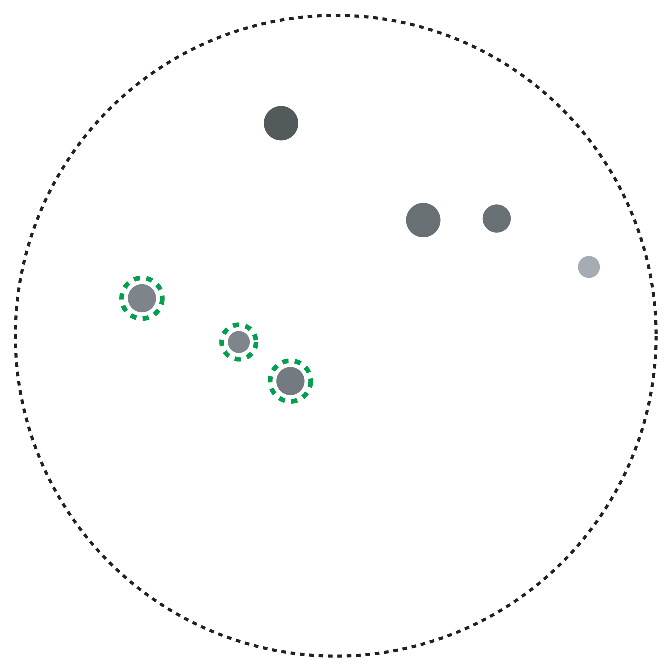
\includegraphics[width=0.31\columnwidth]{misunderstanding_A.pdf}};
	\node[inner sep=0pt] (agent_1) at (4.5,0)
	  {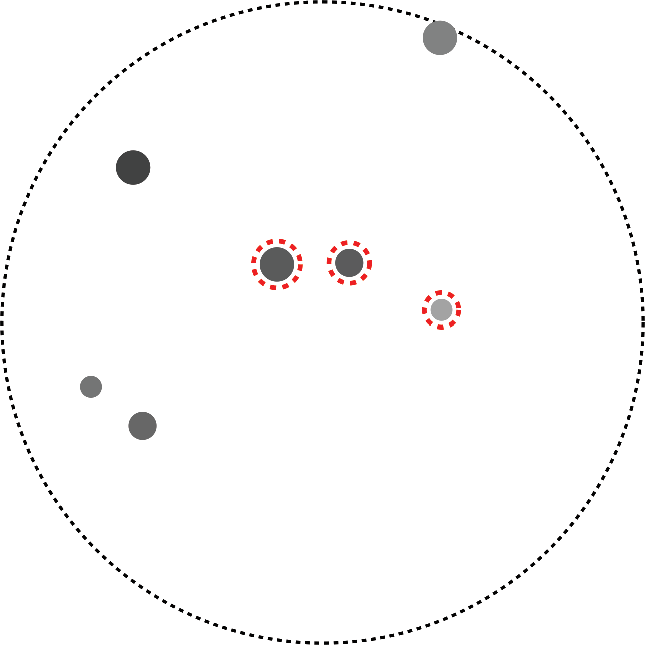
\includegraphics[width=0.31\columnwidth]{misunderstanding_B.pdf}};
	\node [below] at (0,-2.2) {A's View};
	\node [below] at (4.5,-2.2) {B's View};
	\end{tikzpicture} \\[-10pt]
	&
	\small
	\begin{tabular}[t]{@{}l@{}}
	\toprule
	A: I see {\color{mygreen} \underline{\textbf{three smaller circles}}} almost in a line slanting down\\
	from right to left \\
	B: I think I see {\color{myred} \underline{\textbf{it}}}.  Is \underline{the left one} the largest? ... \\
	\bottomrule
	\end{tabular}
	\vspace{6mm}\\
	\raisebox{50pt}{\multirow{2}{*}{{\color{myblue} \textbf{Partial Understanding}}}} & 
	\begin{tikzpicture}
	\node[inner sep=0pt] (agent_0) at (0,0)
	  {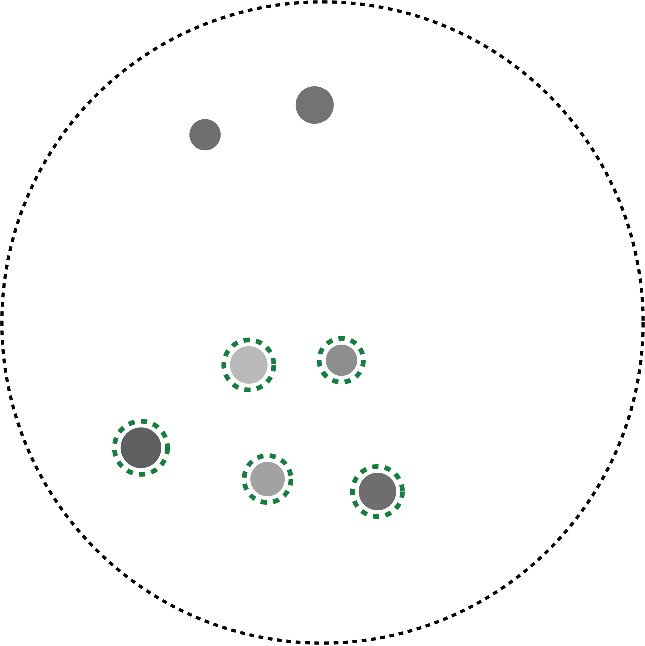
\includegraphics[width=0.31\columnwidth]{partial_understanding_A.pdf}};
	\node[inner sep=0pt] (agent_1) at (4.5,0)
	  {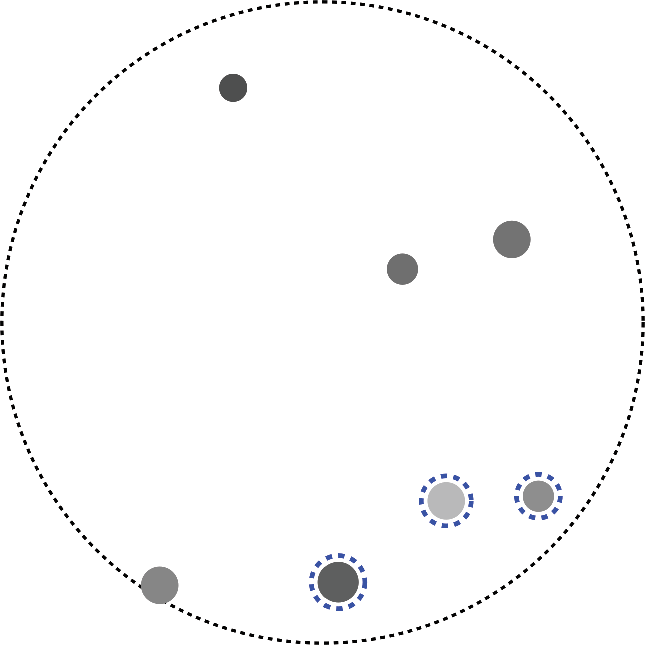
\includegraphics[width=0.31\columnwidth]{partial_understanding_B.pdf}};
	\node [below] at (0,-2.2) {A's View};
	\node [below] at (4.5,-2.2) {B's View};
	\end{tikzpicture} \\[-10pt]
	&
	\small
	\begin{tabular}[t]{@{}l@{}}
	\toprule
	A: I have  {\color{mygreen} \underline{\textbf{5 larger dots}}} close together, \underline{the bottom left one}\\
	is largest and darkest? \\
	B: i have {\color{myblue} \underline{\textbf{three}}} that could be part of that ... \\
	\bottomrule
	\end{tabular}
	\vspace{2mm}
\end{tabular}
}
\caption{Illustrative examples of misunderstanding and partial understanding captured by our annotation.}
\label{04_fig:misunderstanding_partial_understanding}
\end{figure*}

\begin{figure*}[tb!]
\centering
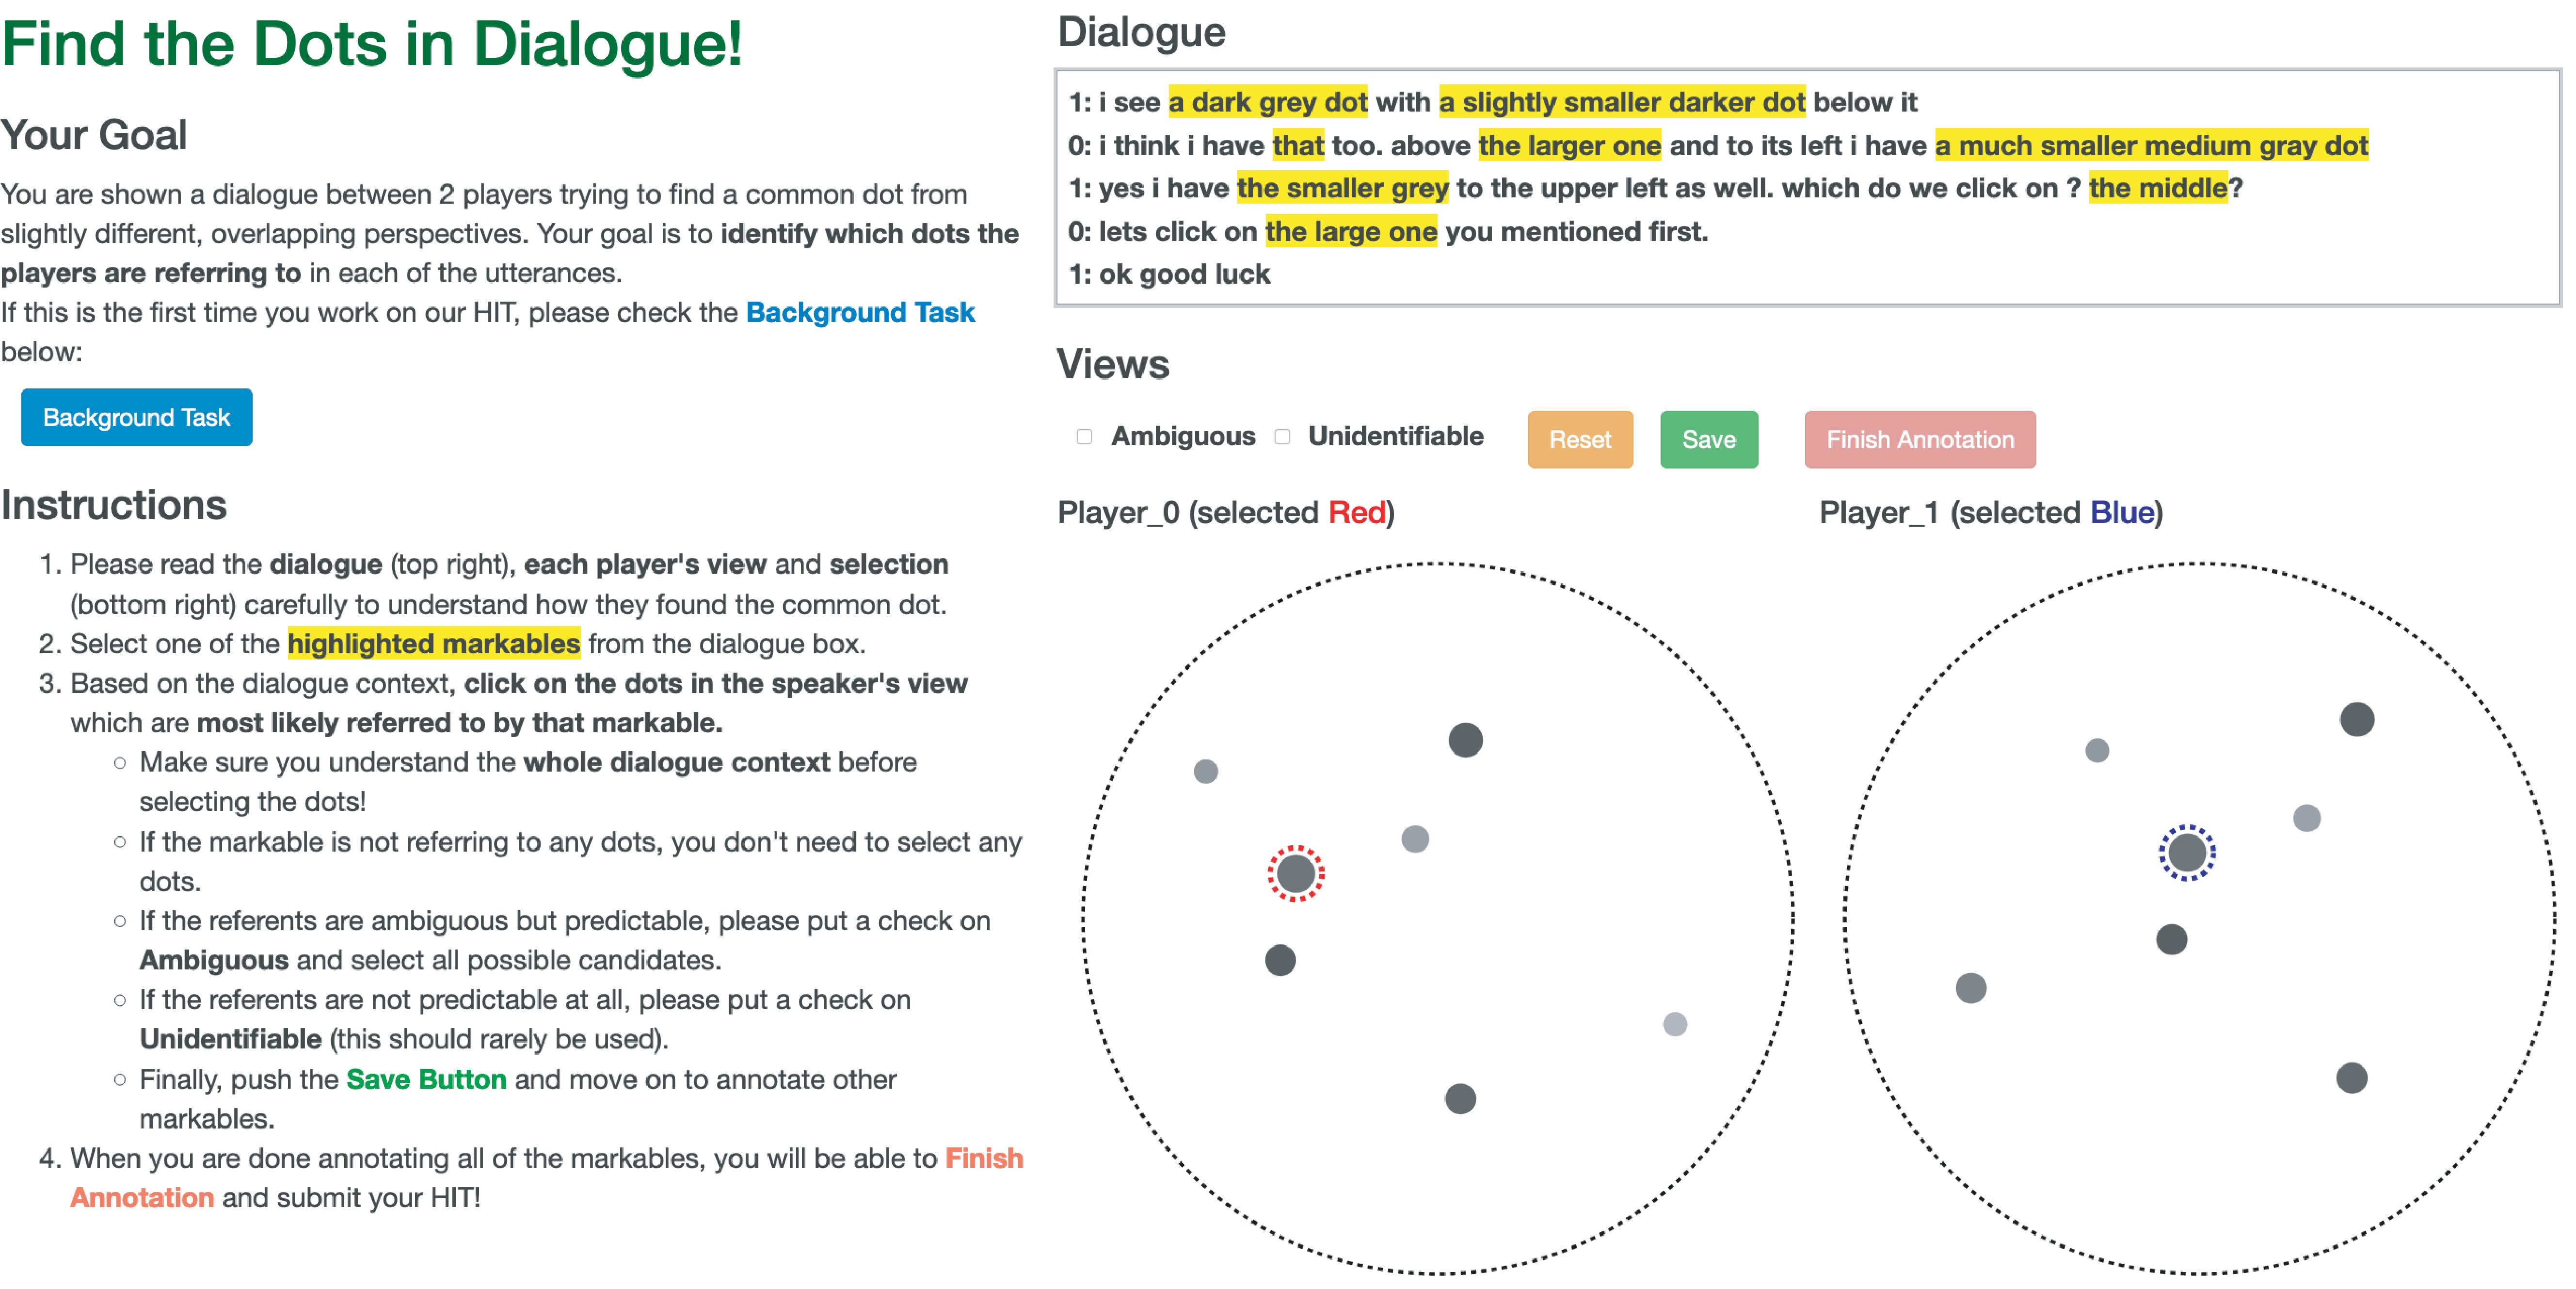
\includegraphics[width=\textwidth]{referent_identification.pdf}
\caption{Our visual interface used for referent identification.}
\label{04_fig:referent_identification_interface}
\end{figure*}


\section{Annotation Results}
\label{04_sec:annotated_corpus}

\subsection{Annotation Statistics}
\label{04_subsec:agreement_statistics}

First, we report the annotation statistics of markable detection in Table \ref{markable_detection_statsitics} and referent identification in Table \ref{04_tab:referent_identification_statistics}. All agreements are computed based on pairwise judgements, and we use Fleiss's Multi-$\pi$ \citep{fleiss1971measuring} to remove the effect of chance level agreements. For markable detection, agreement is calculated for the markable text span (start/end positions at the token level) based on 130 dialogues by 3 annotators. Agreements for markable attributes and relations were also reasonable, but we omit the results since they were optional and used only for the purpose of automatic referent identification. For referent identification, agreement is calculated at the entity-level (whether each entity is included in the referents) and the exact match rate at the markable-level (whether the set of referents match exactly).

Overall, we found high agreement for all annotations (including the crowdsourcing step), which verified the reliability of our annotation framework.

\begin{table*}[t!]
\centering \scalebox{0.78}{
\setlength\tabcolsep{5pt}
\begin{tabular}{ccccccc}
\toprule
\raisebox{-3pt}{\multirow{2}{*}{\# Markables}} & \raisebox{-3pt}{\multirow{2}{*}{\# All-Referents}} & \raisebox{-3pt}{\multirow{2}{*}{\# No-Referent}} & \raisebox{-3pt}{\multirow{2}{*}{\# Anaphora}} & \raisebox{-3pt}{\multirow{2}{*}{\# Cataphora}} & \multicolumn{2}{c}{Agreement (\%)} \\
\cmidrule{6-7}
 & & & & & Start Pos. & End Pos. \\
\midrule
40,172 & 128 & 1,149 & 4,548 & 6 & 99.11 (96.32) & 99.06 (96.11) \\
\bottomrule
\end{tabular}
}
\caption{\label{markable_detection_statsitics}
Annotation statistics for markable detection. Agreement is calculated at the token level (Fleiss's Multi-$\pi$ shown in parenthesis).
}
\end{table*}

\begin{table*}[t!]
\centering \scalebox{0.78}{
\begin{tabular}{cccccc}
\toprule
\# Markables & \# Judgements & Ambiguous (\%) & Unidentifiable (\%) & Agreement (\%) & Exact Match (\%)\\
\midrule
34,341 & 103,894 & 4.65 & 0.77 & 96.26 (88.66) & 86.90 \\
\bottomrule
\end{tabular}
}
\caption{\label{04_tab:referent_identification_statistics}
Annotation statistics for referent identification, along with the rate of \textit{ambiguous} and \textit{unidentifiable} checked in the judgements. Agreement is calculated at the entity-level (Fleiss's Multi-$\pi$ in parenthesis) and exact match rate at the markable-level.
}
\end{table*}

\subsection{Disagreement Analysis}
\label{04_subsec:disagreement_analysis}

\begin{figure}[th!]
\centering
\begin{tikzpicture}
\node[inner sep=0pt] (agent_0) at (0,0)
  {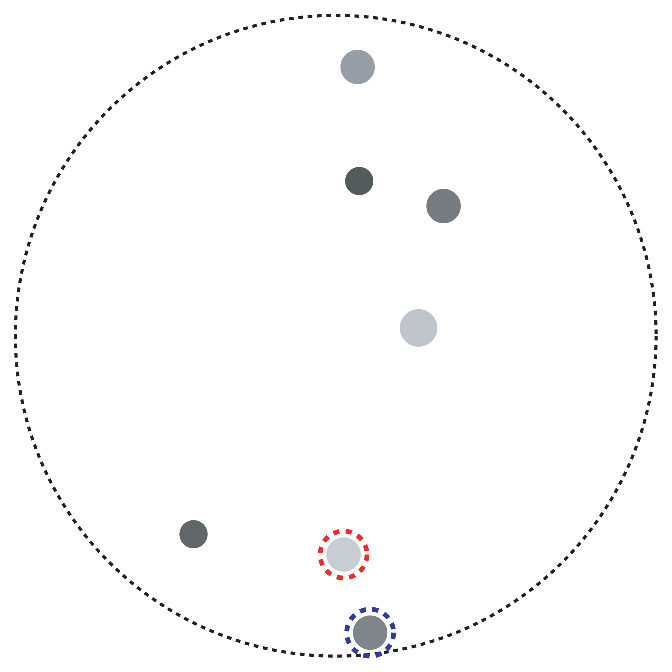
\includegraphics[width=0.3\textwidth]{disagreement_0.pdf}};
\node[inner sep=0pt] (agent_1) at (4.2,0)
  {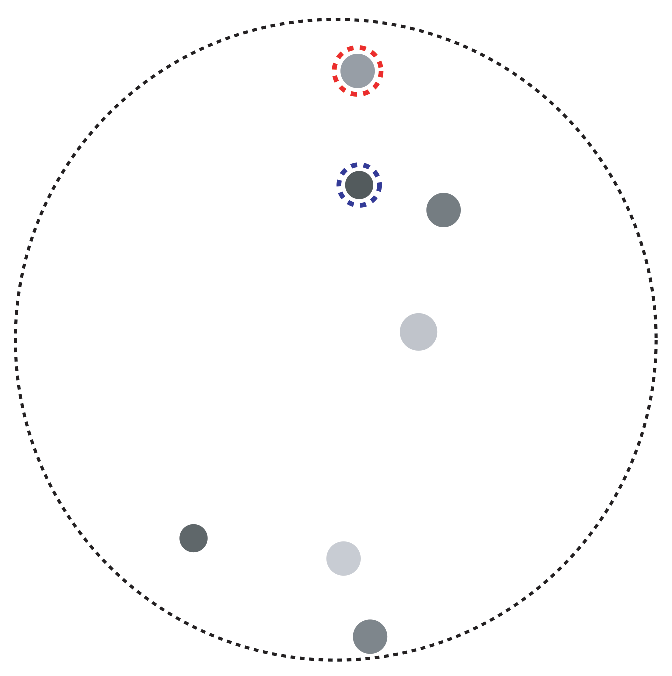
\includegraphics[width=0.3\textwidth]{disagreement_1.pdf}};
\node [below] at (0,3) {Annotator 1};
\node [below] at (4.2,3) {Annotator 2};
\node[text width=8cm] [below] at (2.1,-2.2) {{\color{myred} \underline{\textbf{medium sized light gray dot}}} with {\color{myblue} \underline{\textbf{a darker one}}} directly under {\color{myred} \underline{\textbf{it}}} and to the right? \\};
\end{tikzpicture}
\caption{An example of seemingly reasonable disagreement captured by our annotation.
}
\label{fig:reasonable_disagreement}
\end{figure}

However, it is natural that there is a certain degree of disagreement in referent interpretations. In fact, it is important to capture such disagreements as there can be genuine ambiguity and uncertainty under continuous and partially-observable context (see Figure \ref{fig:reasonable_disagreement} for an example). Therefore, in addition to \textit{explicitly} annotating the ambiguity and unidentifiability (as described in Section \ref{04_subsec:referent_identification}), we aim to capture them \textit{implicitly} by collecting multiple judgements from different annotators.

To study such disagreements in detail, we computed the agreement statistics (e.g. entity-level agreement) conditioned on \textit{the number of referents} in each judgement. To be specific, given a number of referents (from 0 to 7), we collected all judgements with that number of referents and computed the average pairwise agreements with all other judgements on the same markable. The results are summarized in Table \ref{num_referent_agreement}.

\begin{table}[t!]
\centering \scalebox{0.8}{
\setlength\tabcolsep{8pt}
\setlength{\aboverulesep}{0pt}
\setlength{\belowrulesep}{0pt}
\setlength{\extrarowheight}{.3ex}
\begin{tabular}{c|cc|c}
\toprule
\# Referents & Agreement (\%) & Exact Match (\%) & Judgements (\%) \\
\midrule
0 & 78.04 & 17.78 & \phantom{0}1.31 \\
1 & 97.45 & 90.28 & 71.81 \\
2 & 94.87 & 82.17 & 14.85 \\
3 & 93.93 & 83.03 & \phantom{0}7.51 \\
4 & 92.18 & 76.66 & \phantom{0}2.20 \\
5 & 90.31 & 71.03 & \phantom{0}0.88 \\
6 & 90.75 & 78.14 & \phantom{0}1.22 \\
7 & 81.47 & 62.50 & \phantom{0}0.21 \\
\bottomrule
\end{tabular}
}
\caption{\label{num_referent_agreement}
Agreement statistics conditioned on the number of referents (and the percentages of such judgements).
}
\end{table}

We can see that there is a significant amount of disagreements when the number of referents was judged to be 0 (none) or 7 (all). This could be due to several reasons: obvious cases were already annotated as \textit{no-referent} or \textit{all-referents} during markable detection (so only difficult cases were left), annotators simply made mistakes (e.g. forgot to annotate), or the referents were annotated as such when it was too difficult to identify them (e.g. all entities were potential referents). Since the number of such judgements were relatively small, their effect can be mitigated after appropriate aggregation of multiple judgements. We also expect that they provide a useful resource for studying disagreements caused by either the \textit{annotation error} or \textit{genuine ambiguity}, which is a critical problem when multiple interpretations are possible \citep{poesio-etal-2019-crowdsourced}.

In addition, we found that the exact match rate is the highest when the referent is only 1 and much lower as the number of referents increases. This is reasonable because referring expressions of multiple entities tend to be more pragmatic and ambiguous (e.g. \textit{``a cluster"}, \textit{``most of"}, \textit{``a line"}), and it would be more difficult to match the referents exactly. Note that entity-level agreements are still at a high level, and the interpreted referents seem to mostly overlap with each other.

Finally, to study which expressions tend to have higher (or lower) disagreements, we computed the correlations between the occurrence of common tokens (in the markable text) and the exact match rate (of the pairwise judements for the markable). Illustrative examples are shown in Table \ref{token_agreement_corrleation}.

\begin{table}[htb!]
\centering \scalebox{0.8}{
\setlength\tabcolsep{8pt}
\setlength{\aboverulesep}{0pt}
\setlength{\belowrulesep}{0pt}
\setlength{\extrarowheight}{.1ex}
\begin{tabular}{cc}
\begin{tabular}{c|cc}
\toprule
Low & $\rho$ & \# Count \\
\midrule
\textit{it} & -0.149 & 12.7K \\
\textit{any} & -0.103 & \phantom{0}0.5K \\
\textit{that} & -0.100 & 12.5K \\
\textit{your} & -0.083 & \phantom{0}1.5K \\
\textit{few} & -0.081 & \phantom{0}0.1K \\
\textit{what} & -0.081 & \phantom{0}0.4K \\
\textit{others} & -0.064 & \phantom{0}0.8K \\
\textit{line} & -0.062 & \phantom{0}1.7K \\
\textit{bunch} & -0.060 & \phantom{0}0.2K \\
\textit{all} & -0.048 & \phantom{0}1.1K \\
\textit{triangle} & -0.046 & \phantom{0}2.5K \\
\textit{some} & -0.042 & \phantom{0}0.2K \\
\textit{medium} & -0.041 & 12.5K \\
\textit{another} & -0.039 & \phantom{0}1.4K \\
\textit{and} & -0.029 & \phantom{0}1.7K \\
\bottomrule
\end{tabular}
&
\begin{tabular}{c|cc}
\toprule
High & $\rho$ & Count \\
\midrule
\textit{lower} & 0.028 & \phantom{0}1.3K \\
\textit{two} & 0.030 & 14.7K \\
\textit{three} & 0.031 & \phantom{0}4.2K \\
\textit{darkest} & 0.036 & \phantom{0}2.1K \\
\textit{larger} & 0.039 & \phantom{0}7.7K \\
\textit{middle} & 0.041 & \phantom{0}2.1K \\
\textit{smallest} & 0.043 & \phantom{0}2.0K \\
\textit{very} & 0.056 & \phantom{0}6.1K \\
\textit{top} & 0.061 & \phantom{0}5.2K \\
\textit{light} & 0.072 & 18.7K \\
\textit{tiny} & 0.076 & \phantom{0}7.8K \\
\textit{large} & 0.084 & 21.7K \\
\textit{the} & 0.125 & 55.0K \\
\textit{one} & 0.136 & 57.1K \\
\textit{black} & 0.145 & 26.9K \\
\bottomrule
\end{tabular}
\end{tabular}
}
\caption{\label{token_agreement_corrleation}
Tokens with low or high correlation with the exact match rate (Pearson's correlation coefficient shown in $\rho$).
}
\end{table}

In general, the correlations are very small and the amount of disagreements seem relatively constant across all token types. However, the general trend is still intuitive: ambiguous or complex expressions such as pronouns, interrogatives, quantifiers, and conjunctions tend to have negative correlations, while simple and plain expressions tend to have positive correlations.

To summarize the analysis, our annotation has high overall agreement but also includes interesting, reasonable disagreements which capture the ambiguity and uncertainty under continuous and partially-observable context.

\subsection{Pragmatic Expressions}
\label{04_subsec:pragmatic_expressions}

Finally, we give an illustrative example of additional analyses that can be conducted based on our annotation. To be specific, we give a more quantitative analysis of \textit{pragmatic expressions} which we introduced as a characteristic strategy under continuous context (Section \ref{03_subsec:difficulty_analysis}).

\begin{figure}[ht]
\centering
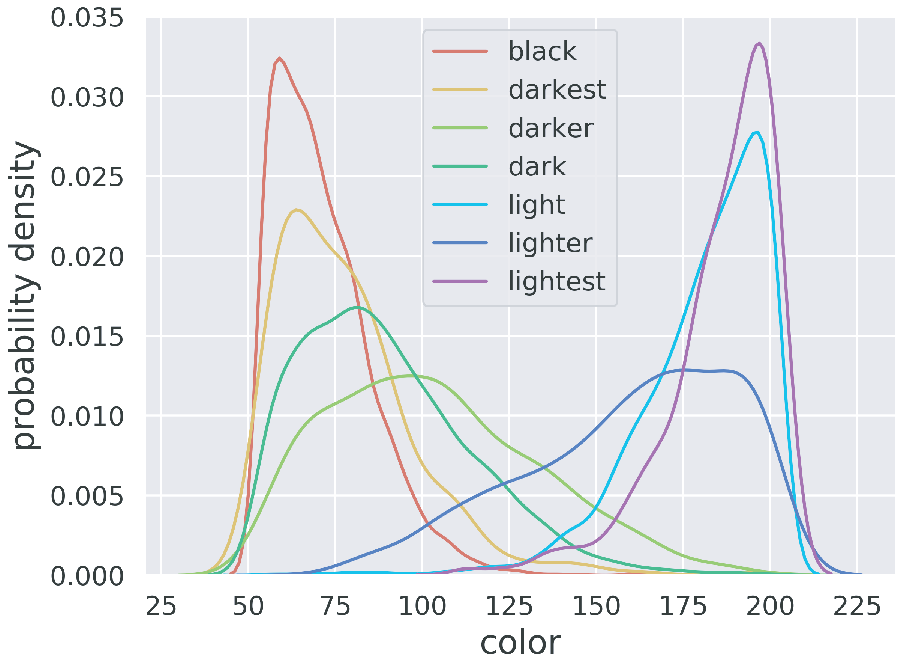
\includegraphics[width=0.7\textwidth]{color_distplot_cmyk.pdf}
\caption{Distributions of the actual color of the referents expressed by common adjectives (the range of color is 256 in grayscale, lower is darker).}
\label{fig:color_distplot}
\end{figure}

As an illustration, we focus on the pragmatic expressions of \textit{color} and estimate the distributions of the actual color of the referents described by the common adjectives. We simply assume that the adjective in the markable (minimal noun phrase) describes the color of the referents, since the exceptions (such as negation in the prenominal modifier) seemed rare and ignorable. For the sake of visualization, empirical distributions are smoothed based on kernel density estimation. As we can see in Figure \ref{fig:color_distplot}, all adjectives (including the specific color ``black'') have relatively wide distributions which overlap with each other. This is a strong evidence that the color expressions are pragmatic, i.e. the same adjective can be used for different colors (and in return, the same color can be described in different ways) depending on the context.


\section{Experiments}
\label{04_sec:experiments}

In this experiment, we evaluate and analyze baseline dialogue models based on the following three tasks: 

\begin{itemize}
  \item First is the \textbf{target selection task} from Chapter \ref{03_chp:task_formulation}, where the model predicts the target entity selected by each player at the end of collaborative reference. This task requires accurate recognition of the created common ground.
  \item Second is the \textbf{reference resolution task}, where the model predicts the referent entities for each markable in the dialogue. Note that the model is given only one player's observation and predicts the markables in that player's utterances only. This task requires accurate comprehension of the intermediate process of common grounding.
  \item Last is the \textbf{selfplay dialogue task}, where the model plays the whole collaborative reference task against an identical copy of itself. This requires the actual creation of common ground through natural language communication, despite against the copy of itself (and not with real humans).
\end{itemize}

To create the golden labels for reference resolution, we used simple majority voting based on the multiple judgements or automatically identified the referents based on markable attributes/relations. Note that markables were removed if the majority considered their referents as unidentifiable (in the referent identification step).

%If the referents were considered unidentifiable by the majority in step 2 (referent identification), we removed such markables from the dataset

%Note that markables were removed if the majority considered their referents as unidentifiable.

\subsection{Model Architecture}
\label{04_subsec:model_architecture}

\begin{figure*}[th]
\centering
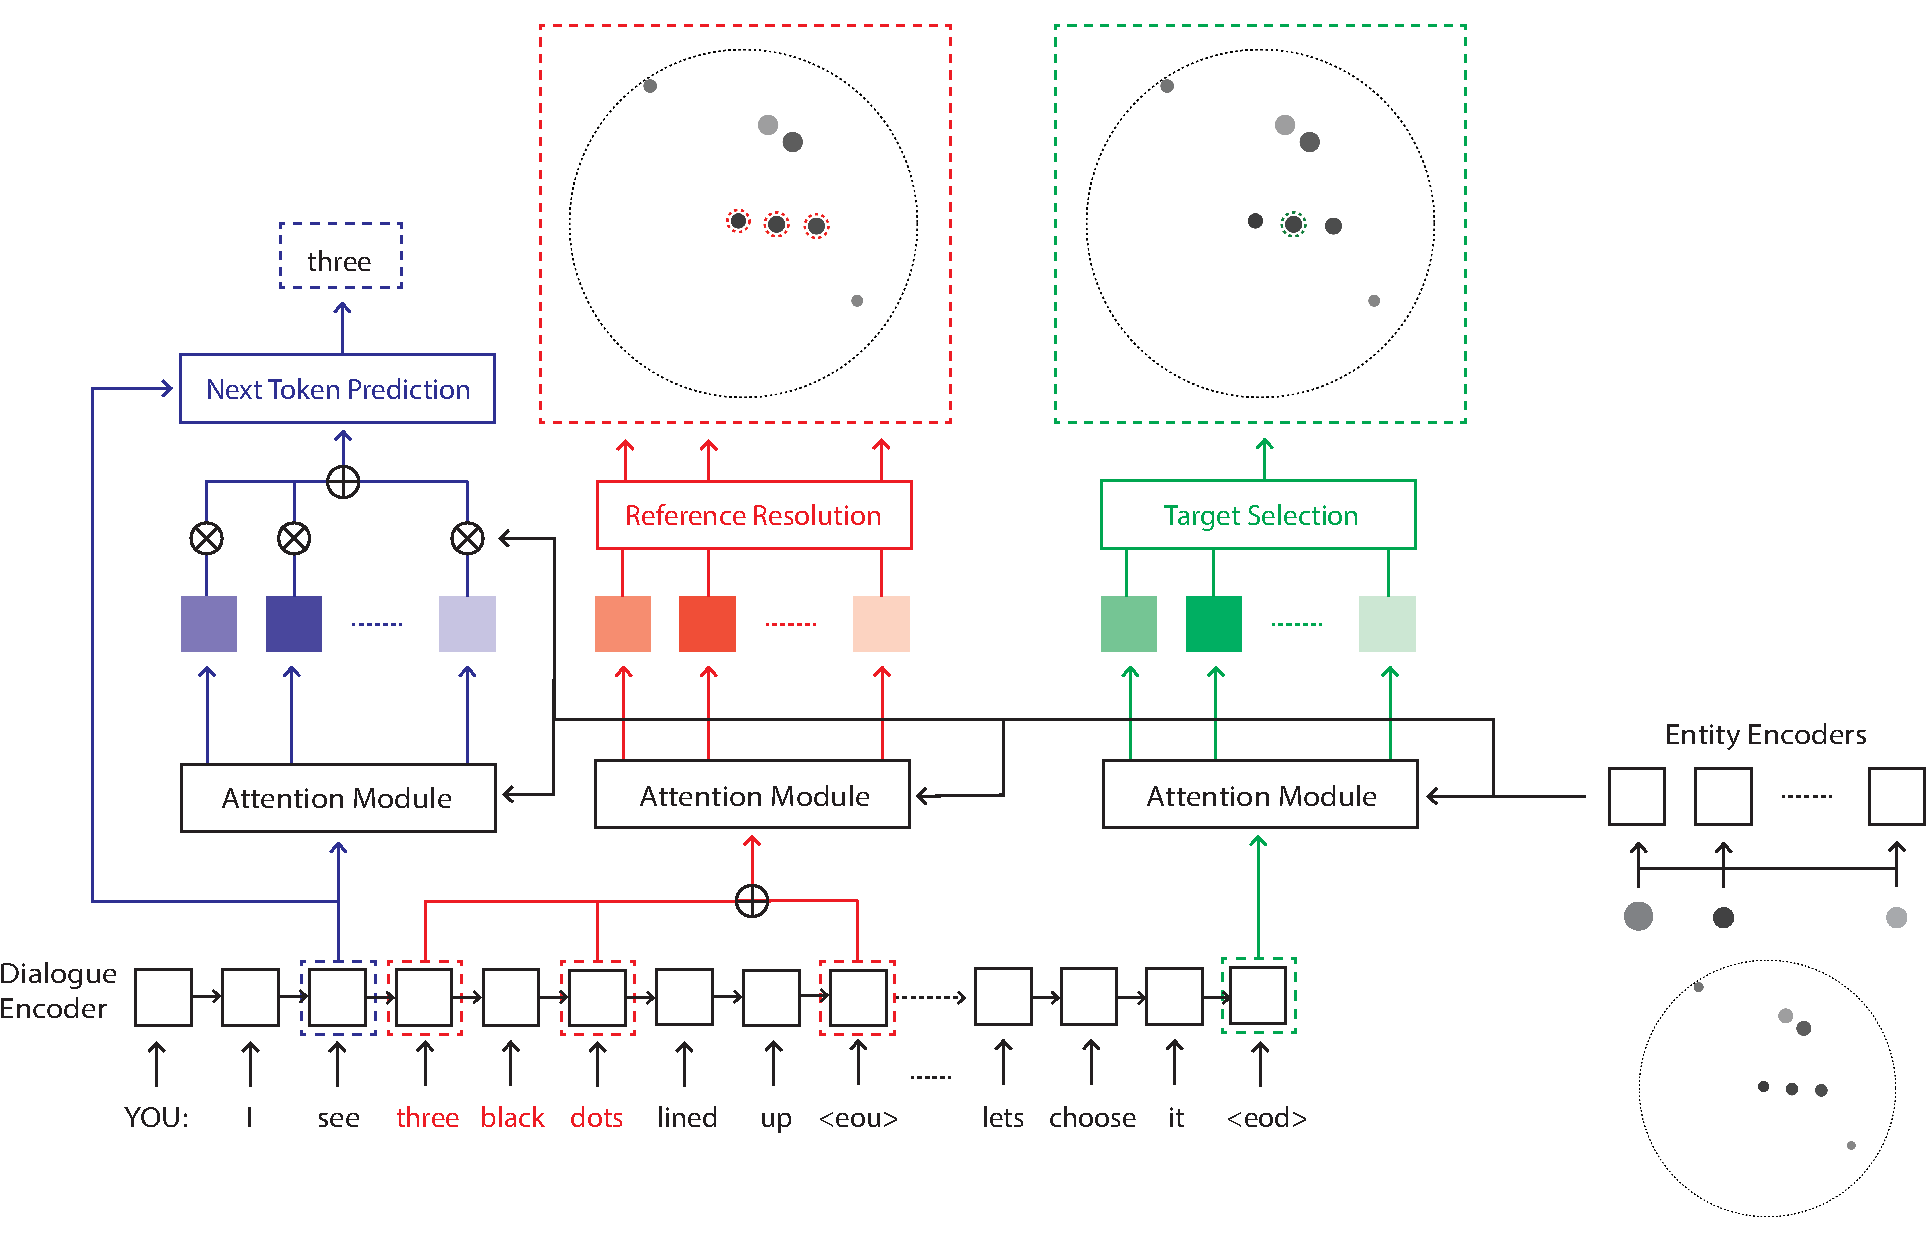
\includegraphics[width=\textwidth]{model_architecture.pdf}
\caption{Our baseline model architecture (best seen in color). TSEL decoder is shown in green, REF decoder and the input markable (``three black dots'') are in red, and DIAL decoder is in blue. All decoders share (some or all layers of) the attention module.}
\label{fig:model_architecture}
\end{figure*}

The overall architecture of our baseline end-to-end models is shown in Figure \ref{fig:model_architecture}.

\subsubsection{Encoders}

Our baseline models have two encoders: one for encoding dialogue tokens and one for context information.

Dialogue tokens are encoded based on a unidirectional GRU \citep{cho2014properties}. To encode context information, we use a shared \textit{entity encoder} to create entity-level representations of the context. This consists of two modules: an \textit{attribute encoder} which encodes the attributes of each entity (size, color and 2-D location) with a matrix followed by a tanh layer, and a \textit{relational encoder} which encodes relative attributes of each entity pairs with another matrix followed by a tanh layer. The final representation of each entity is the concatenation of its attribute encoding and the sum of relational encodings with the other 6 entities. Note that we refined the method from Chapter \ref{03_chp:task_formulation}, where the context is encoded into a single representation (and not entity-level representations).

%a \textit{relational encoder} which embeds pairs of entity attributes with another matrix followed by a tanh layer. The final embedding of each entity is the concatenation of its attribute embedding and the sum of relational embeddings with the other 6 entities.

\subsubsection{Decoders}

Our models can have up to three decoders: TSEL for target selection, REF for reference resolution, and DIAL for predicting next dialogue tokens. Each decoder shares (some or all layers of) the \textit{attention module} based on an MLP which computes a scalar score for each entity. Specifically, this module takes the representation of each entity and the following positions (states) of the GRU as the input: the \textit{final hidden state} for TSEL, the \textit{start/end positions of the markable} and the \textit{end position of the utterance} for REF, and the \textit{current hidden state} for DIAL. Based on the computed attention scores, TSEL simply computes the softmax and REF computes logistic regressions for each entity. DIAL reweights the entity representations based on their attention scores to focus on the relevant entities in next token prediction \citep{bahdanau2014nmt,xu2015show}.\\

In this experiment, we built five models based on different combinations of the three decoders. All models are trained with the same default hyperparameters, following the similar setup as Chapter \ref{03_chp:task_formulation}.


\subsection{Results}
\label{04_subsec:results}

\begin{table*}[tb!]
\centering \scalebox{0.77}{
\setlength\tabcolsep{6pt}
\setlength{\aboverulesep}{0pt}
\setlength{\belowrulesep}{0pt}
\setlength{\extrarowheight}{.3ex}
\begin{tabular}{c|cccccc}
\toprule
\multirow{2}{*}{Model} & \multirow{2}{*}{Target Selection} & Reference Resolution & \multicolumn{3}{c}{Selfplay Dialogue} \\
 & & (Accuracy / Exact Match) & \#Shared=4 & \#Shared=5 & \#Shared=6 \\
\midrule
TSEL & 67.79{\scriptsize $\pm$1.53}  & -  & - & - & - \\
REF & - & \textbf{85.75{\scriptsize $\pm$0.22}} / \textbf{33.91{\scriptsize $\pm$0.86}} & - & - & - \\
TSEL-REF & \textbf{69.01{\scriptsize $\pm$1.58}} & 85.47{\scriptsize $\pm$0.36} / 32.88{\scriptsize $\pm$1.28} & - & - & - \\
\midrule
TSEL-DIAL & 67.01{\scriptsize $\pm$1.29} & - & 42.07{\scriptsize $\pm$1.27} & 57.37{\scriptsize $\pm$1.29} & 77.00{\scriptsize $\pm$1.13} \\
TSEL-REF-DIAL & \textbf{69.09{\scriptsize $\pm$1.12}} & 85.86{\scriptsize $\pm$0.18} / 33.66{\scriptsize $\pm$0.93} & \textbf{45.78{\scriptsize $\pm$2.15}} & \textbf{61.95{\scriptsize $\pm$1.72}} & \textbf{80.01{\scriptsize $\pm$1.61}} \\
\midrule
Human & 90.79 & 96.26 / 86.90 & 65.83 & 76.96 & 87.00 \\
\bottomrule
\end{tabular}
}
\caption{\label{04_tab:baseline_results}
Results of our experiments. For reference resolution, \textit{accuracy} is computed at the entity-level and \textit{exact match rate} at the markable-level. Human scores are taken from Table \ref{03_tab:statistics} and \ref{04_tab:referent_identification_statistics} as a reference.
}
\end{table*}

We run the experiments 10 times with different random seeds and dataset splits. For selfplay dialogues, we generated 1,000 scenarios with each number of shared entities (4, 5 or 6) and set the output temperature to 0.25 during next token prediction. We report the mean and standard deviation of the results in Table \ref{04_tab:baseline_results}.

In terms of \textit{target selection} and \textit{selfplay dialogue} tasks, we found consistent improvements by training the models jointly with reference resolution (i.e. with REF decoder). This verified that even simple multi-task training with the central subtask can improve performance on difficult end tasks. The results for \textit{reference resolution} are reasonably high in terms of entity-level accuracy but much lower in terms of exact match rate. Considering the high agreements (Section \ref{04_subsec:agreement_statistics}) and improved reliability of the gold annotation after aggregation, we expect there to be a huge room for further improvements.

Overall, common grounding under continuous and partially-observable context is still a challenging task, and we expect our resource to be fundamental for solving this task along with the accurate capability of reference resolution.

\subsection{Further Analysis}
\label{subsection:analysis}

To demonstrate the advantages of our annotation for interpreting and analyzing dialogue systems, we give a more detailed analysis of TSEL-REF-DIAL model which performed well on all three tasks. In Table \ref{04_tab:exact_match_results}, we show the results for reference resolution grouped by the number of referents in the gold annotation. In terms of the exact match rate, we found that the model performs very well on 0 and 7 referents: this is because most of them can be recognized at the superficial level, such as ``\underline{none of them}", ``\underline{all of mine}", ``I don't have \underline{that}", etc. However, the model struggles on all other cases: the results are especially worse for markables with more than one referent. This shows that the model still lacks the ability of precisely tracking multiple referents, which can be expressed in complex, pragmatic ways (based on the grouping strategies).

In addition, we found that the correlation between the reference resolution accuracy (i.e. average accuracy of reference resolution in each dialogue) and the target selection accuracy (i.e. binary result of target selection in each dialogue) was relatively weak, with an average of only $0.23$ in the 10 runs of the experiments. This reveals that the model is often correct for the target selection task based on the \textit{wrong reason}, without tracking the referents correctly \citep{mccoy-etal-2019-right}. Our annotation is also useful for error analyses in recognizing common ground, e.g. by inspecting \textit{where} the model made a mistake and lost track of the correct referents.


\begin{table}[th]
\centering \scalebox{0.96}{
\small
\setlength\tabcolsep{8pt}
\setlength{\aboverulesep}{0pt}
\setlength{\belowrulesep}{0pt}
\setlength{\extrarowheight}{.3ex}
\begin{tabular}{c|cc|c}
\toprule
\# Referents & Accuracy (\%) & Exact Match (\%) & \# Count \\
\midrule
0 & 95.91{\scriptsize $\pm$1.38} & 83.53{\scriptsize $\pm$4.65}\phantom{0} & \phantom{0}148.5 \\
1 & 89.34{\scriptsize $\pm$0.17} & 36.86{\scriptsize $\pm$1.32}\phantom{0} & 2782.5 \\
2 & 78.14{\scriptsize $\pm$1.07} & 20.59{\scriptsize $\pm$1.90}\phantom{0} & \phantom{0}587.9 \\
3 & 70.64{\scriptsize $\pm$1.02} & 13.63{\scriptsize $\pm$2.06}\phantom{0} & \phantom{0}283.3 \\
4 & 69.12{\scriptsize $\pm$2.69} & 10.16{\scriptsize $\pm$3.47}\phantom{0} & \phantom{00}81.0 \\
5 & 73.57{\scriptsize $\pm$2.94} & 17.56{\scriptsize $\pm$5.88}\phantom{0} & \phantom{00}33.0 \\
6 & 78.69{\scriptsize $\pm$4.45} & 13.18{\scriptsize $\pm$7.31}\phantom{0} & \phantom{00}43.0 \\
7 & 74.60{\scriptsize $\pm$7.49} & 50.38{\scriptsize $\pm$11.40} & \phantom{00}22.3 \\
\bottomrule
\end{tabular}
}
\caption{\label{04_tab:exact_match_results}
Detailed results for the reference resolution task grouped by the number of referents in the gold annotation (along with the average counts in the test set).
}
\end{table}


\begin{figure}[th!]
\centering
\begin{tikzpicture}
\node[inner sep=0pt] (agent_0) at (0,0)
  {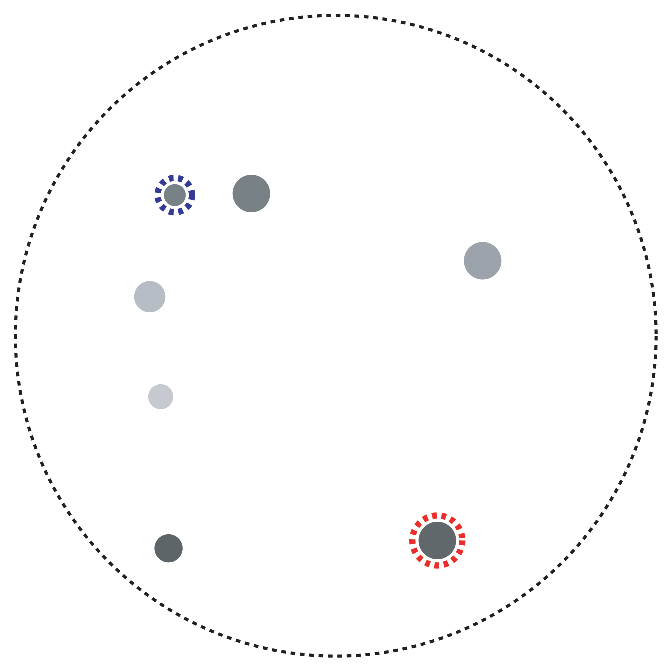
\includegraphics[width=0.3\textwidth]{selfplay_alice.pdf}};
\node[inner sep=0pt] (agent_1) at (4.2,0)
  {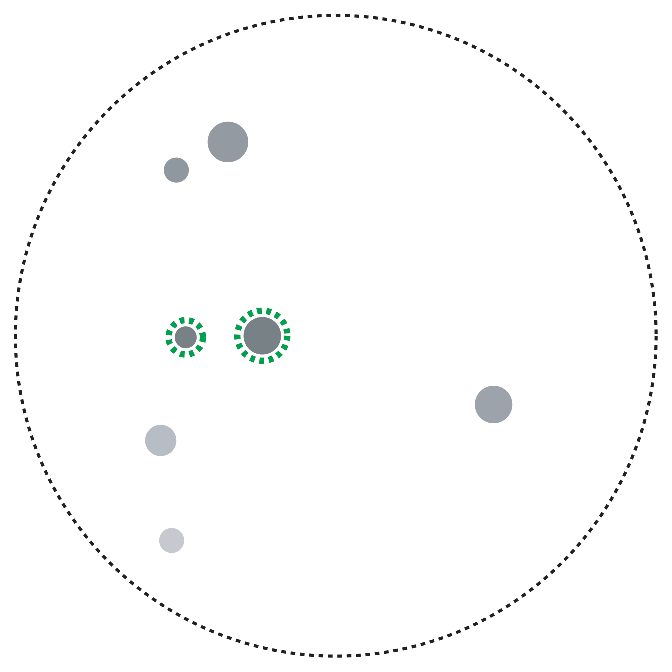
\includegraphics[width=0.3\textwidth]{selfplay_bob.pdf}};
\node [below] at (0,-2) {Model A's view};
\node [below] at (4.2,-2) {Model B's view};
\end{tikzpicture}
\small
\begin{tabular}{l}
\toprule
A: I have {\color{myred} \underline{\textbf{a large black dot}}} with {\color{myblue} \underline{\textbf{a smaller dark dot}}} to the\\ right of {\color{myred} \underline{\textbf{it}}} \\
B: I see {\color{mygreen} \underline{\textbf{that}}} . Let's pick \underline{the large black dot} \\
\bottomrule
\end{tabular}
\caption{An example dialogue from the selfplay dialogue task by the TSEL-REF-DIAL model. Predicted referents are highlighted (no referents are predicted for ``the large black dot'').
}
\label{fig:selfplay}
\end{figure}

Finally, we show an example dialogue from the selfplay task with the interpreted process of common grounding (Figure \ref{fig:selfplay}). Referring expressions are automatically detected by a BiLSTM-CRF tagger \citep{huang2015bidirectional} trained on our corpus with the result of 98.9\% accuracy at the token level. Based on the raw dialogue only, it is difficult to identify which entities model A is referring to. However, by visualizing the intended referents, we can see that model A is describing two entities in somewhat unnatural and inappropriate way (albeit using the anaphoric expression ``it'' appropriately). We can also verify that model B acknowledges this in a perfectly coherent way but without predicting any referent for ``the large black dot'': we often observed such phenomena, where the utterance by a model cannot be interpreted correctly \textit{even by itself}. Overall, our annotation allows for fine-grained analysis of both the \textit{capabilities} and \textit{incapabilities} of existing dialogue systems. The generated dialogue is short in this example, but our approach would be even more critical for interpretation as the dialogues get longer and more complicated.

\section{Related Work}
\label{03_sec:related_work}

Coreference and anaphora resolution have been studied extensively in NLP \citep{pradhan2011conll,poesio2016anaphora}, including disagreements in their interpretations \citep{recasens-etal-2012-annotating,poesio-etal-2019-crowdsourced}. The main novelty of our annotation schema is the focus on \textit{exophoric references} and direct annotation of the referents in the \textit{external modality}. This allows us to study the aspect of \textit{symbol grounding} in the visual context, as we discuss in the next chapter. This also enables reliable and intuitive annotation, even by using non-expert annotators for referent identifications. Finally, our annotation (at least indirectly) captures basic coreferences as well as complex associative anaphora (such as \textit{part-of} relations): with additional annotations, we can also capture more fine-grained, explicit relations between anaphora as well.

Our work is also relevant to the recent literature of interpretable and explainable machine learning \citep{doshi2017towards,lipton2016mythos}. Especially the analysis of neural based models is gaining attention in NLP \citep{belinkov-glass-2019-analysis}, including end-to-end dialogue models \citep{sankar-etal-2019-neural}. The main novelty of our approach is that we decompose the original task (\textit{common grounding}) based on its central subtask (or could be subtasks), define the subtask (\textit{reference resolution}) formally with an annotation framework, and create a large-scale resource to study the subtask along with the original task. Our approach has several advantages compared to previous analysis methods. First, it is applicable to \textit{both humans and machines}, which is especially important in dialogue domains where they interact. Second, it can be used to study the \textit{relationships} between the original task and its subtasks, which is critical for a more \textit{skill-oriented} evaluation of artificial intelligence \citep{Hernndez-Orallo:2017:MME:3110808,sugawara2017prerequisite}. Third, it can be used for investigating \textit{the dataset} on which the models are trained: this is important in many aspects, such as understanding undesirable biases in the dataset \citep{gururangan-etal-2018-annotation,sugawara-etal-2018-makes} or correct model predictions based on the \textit{wrong reasons} \citep{mccoy-etal-2019-right}. Finally, the collected resource can be used for both \textit{probing} whether the models solve the subtasks implicitly \citep{linzen2016assessing} or \textit{developing} new models which can be explicitly supervised, evaluated and interpreted based on the subtasks.

Finally, visually grounded dialogues have been studied in a wide variety of settings. In comparison, the main strengths and novelty of our (annotated) OneCommon Corpus can be summarized as follows:

\begin{enumerate}[label=(\Alph*)]
  \item Our corpus is based on the advanced setting of continuous and partially-observable context where complex common grounding strategies are introduced.
  \item Our corpus has the simplicity and controllability to make fully controlled experiments and analyses possible.
  \item Our corpus contains large-scale manual annotation of reference resolution and detailed analyses of agreements/disagreements based on multiple judgements.
\end{enumerate}

Prior work in common grounding \citep{potts2012goal,de2017guesswhat} and visual reference resolution \citep{tokunaga-etal-2012-rex,zarriess-etal-2016-pentoref} mostly focus on categorical or fully-observable settings and do not satisfy (A). While visual dialogues based on photographic scenes \citep{das2017visual,haber-etal-2019-photobook,ilinykh2019meetup} have the strengths of being more complex and realistic, they do not satisfy (B). \citet{gotze-boye-2016-spaceref} conducted a smaller-scale annotation of reference resolution but do not assess the reliability of the annotation, hence not satisfying (C). To the best of our knowledge, our work is the first (and only) resource to satisfy all of the above criteria.

\section{Conclusion}
\label{04_sec:conclusion}

One of the most influential models of common grounding to date is the \textit{contribution} model of \citet{clark1989contributing}: however, applying such theory in realistic settings can be difficult or even problematic. In this chapter, we proposed a novel method of decomposing common grounding based on the subtask of reference resolution to study the intermediate process of common grounding. Based on our annotated corpus, we demonstrated the advantages of our approach for analyzing human strategies as well as interpreting and improving baseline (end-to-end) dialogue models. Overall, we expect our study to be a fundamental step towards interpreting and improving common grounding through reference resolution.
